\documentclass{article}
\usepackage[utf8]{inputenc}
\usepackage[margin=0.8in]{geometry}
\usepackage{graphicx}
\usepackage{wrapfig}

\usepackage{natbib}
\usepackage{graphicx}
% Para los codigos
\usepackage{listings}
\usepackage[spanish]{babel}
\usepackage[hidelinks]{hyperref}
\usepackage{lscape}
\usepackage{rotating}
\usepackage{pdflscape}

\lstset{
basicstyle=\ttfamily,
frame=single,
language=SQL,
tabsize=2,
literate=%
    {á}{{\'a}}1
    {é}{{\'e}}1
    {è}{{\`e}}1
    {í}{{\'i}}1
    {ó}{{\'o}}1
    {ú}{{\'u}}1
}
\begin{document}

\begin{titlepage}
	\title{
		\begin{Huge}
			Practica 3 - BASES DE DATOS 2
		\end{Huge}
	}
	\author{
	  Hayk Kocharyan\\
	  757715@unizar.es
	  \and
	  Juan José Tambo Tambo\\
	  755742@unizar.es
	  \and
	  Pedro Tamargo Allué\\
	  758267@unizar.es
	  \and
	  Jesús Villacampa Sagaste\\
	  755739@unizar.es
	}
	\date{\today}
	
	\clearpage\maketitle
	\thispagestyle{empty}
	\tableofcontents

\end{titlepage}

\newpage 

\section{Esfuerzos invertidos}
Los esfuerzos invertidos por cada integrante del equipo son:
\begin{itemize}
\item Hayk:

\item Juanjo:	

\item Jesús:

\item Pedro: 

\end{itemize}

\section{Parte 1 - Esquema conceptual y lógico de la base de datos relacional diseñada en la práctica anterior}

\textbf{Mostrar aqui el ER de la práctica anterior y contar su traducción a SQL diciendo las decisiones de diseño de forma DETALLADA.}

Durante el desarrollo de la práctica 1 se diseñó una base de datos para un banco que quería gestionar cuentas con múltiples propietarios, diferentes tipos de cuentas (cuentas ahorro y cuentas corrientes), operaciones (transacciones entre cuentas, o movimientos de dinero en efectivo) y las sucursales de la entidad.\\
En la Figura \ref{fig:er1} se puede observar el esquema entidad relación sobre el problema planteado. Se ha planteado las relaciones entre los distintos tipos de cuentas como una generalización, ya que todas comparten ciertos atributos como el número de cuenta, el \emph{IBAN}, la fecha de apertura y el saldo restante. Esta generalización es exclusiva ya que no se considera posible la capacidad de que una cuenta pertenezca a los dos tipos de entidades al mismo tiempo. También, se trata de una generalización total ya que no se considera el caso de que una cuenta no pertenezca a algunos de las entidades derivadas de \emph{Cuenta}.\\
Con transacción ocurre lo mismo, una transferencia entre cuentas y las operaciones de retirada o ingreso de efectivo se pueden generalizar en una nueva entidad \emph{Transacción} con los atributos comunes a ambas entidades, tales como: el número de la transacción, la fecha y hora de la misma, su importe y una descripción a modo de concepto. Se trata de una generalización exclusiva ya que una transferencia no puede pertenecer a los dos subtipos a la vez. También, se trata de una generalización total ya que en el contexto del problema no tiene sentido que exista una transferencia que no pertenezca a \emph{Operación (operaciones en efectivo)} o a \emph{Transferencia (transferencia de saldo entre cuentas)}.\\
Se ha decidido que \emph{Transacción} debía ser débil respecto a \emph{cuenta} ya que depende en existencia e identificación de \emph{cuenta}, por lo tanto la relación \emph{Realizar} es una relación \emph{1:N} entre \emph{Cuenta} y \emph{Transacción}. No obstante, existe una transacción que no indica la debilidad de la entidad \emph{Transacción} respecto a \emph{Cuenta}, la relación \emph{Recibir}, una relación \emph{1:N} que relaciona las entidades \emph{Cuenta} y \emph{Transferencia} , y cuyo significado es relacionar una transferencia con la cuenta beneficiaria.\\
Los clientes titulares de una cuenta se reflejan en la entidad \emph{Cliente}, que almacena el DNI, el nombre, los apellidos la dirección y el email. Se ha decidido que el \emph{DNI} sea la clave primaria ya que es único para los ciudadanos.\\
La relación de \emph{Cliente} con \emph{Cuenta} se encuentra en \emph{Poseer}, una relación \emph{M:N} que posibilita que una cuenta tenga más de un titular.\\
Para el almacenamiento de las sucursales de la entidad bancaria, se ha diseñado una entidad \emph{Sucursal}, que almacena el código de la entidad, su dirección postal y el teléfono de la oficina. Se ha decidido que el código de la sucursal sea la clave primaria que identifique a las sucursales ya que dentro de la misma entidad bancaria no existen dos sucursales con el mismo código.\\
Se ha considerado que las transacciones se tienen que realizar en una sucursal, por lo tanto existe una relación entre \emph{Transacción} y \emph{Sucursal}. También, una cuenta corriente debe ser abierta en una determinada sucursal de la entidad.\\

En la traducción de las generalizaciones del esquema conceptual al esquema lógico (modelo relacional) se han escogido dos estrategias. En la generalización de \emph{Cuenta} se ha mantenido la entidad, y las entidades derivadas de la misma solamente almacenan los atributos necesarios que no pertenecen a \emph{Cuenta}.\\
Por otra parte, en la generalización de \emph{Transacción} se ha optado por eliminar la entidad generalizada, obteniendo así dos entidades independientes y duplicando algunos de sus atributos. \textbf{Leyendo esto me doy cuenta que nos hacía falta un \emph{Trigger}}. En esta misma generalización se ha traducido la relación \emph{1:N} entre \emph{Cuenta} y \emph{Transacción} como un atributo (el número de cuenta) en la tablas derivadas de \emph{Transacción} \textbf{TODO: Esto no se cuanto de bien está redactado}, siendo una referencia a la cuenta que ha realizado la transacción.\\
{\LARGE \textbf{¿CÓMO LES PONEMOS EL ESQUEMA LÓGICO? Un diagrama?}}

\section{Parte 1 - Determinación del esquema lógico y conceptual de la base de datos Oracle a integrar}

\textbf{Esquema ER de la base de datos a integrar y PONER LAS CONSULTAS CON LAS QUE HEMOS SACADO LAS COSAS.}\\
\textbf{Igual estaría bien comentar de donde hemos sacado la información.}

En esta práctica se pide integrar la base de datos de la Práctica 1+2 en otra base de datos ya existente (\emph{Banquete}). Para ello, es preciso conocer la organización de sus tablas y como se relacionan unas con otras, por tanto, el primer paso para conseguir la integración es extraer toda la información posible de la base de datos de \emph{Banquete}.\\
\emph{Banquete} es una base de datos proporcionada por los profesores de la asignatura y se puede acceder a ella a través de las máquinas del laboratorio. Al conectarse a \emph{lab000} y ejecutar el comando \emph{sqlplus2 aNIP@barret.danae04.unizar.es} (siendo NIP el identificador de la universidad de cada miembro) e introduciendo la contraseña proporcionada en el fichero \emph{README-oracle2}, cada componente del grupo tiene acceso a Oracle con la base de datos \emph{Banquete} ya cargada.\\
Una vez conseguido el acceso a \emph{Banquete}, a través de las consultas expuestas a continuación se consigue toda la información sobre tablas, vistas, triggers o constraints necesarios para conocer el funcionamiento al completo de la misma. 

\textbf{TODO Hay que insertar todas consultas que hicimos CREO QUE FALTAN}

\begin{lstlisting}
	-- Obtenemos las tablas
	SELECT table_name FROM user_tables@SCHEMA2BD2;
	-- Describir los atributos de la tabla <nombre_tabla>
	DESC <nombre_tabla>@SCHEMA2BD2;

	-- Para obtener las restricciones (clave primaria, ajena,
	--  restricciones de consistencia) para una tabla <nombre_tabla>
	SELECT UCC.CONSTRAINT_NAME, UCC.COLUMN_NAME, UC.CONSTRAINT_TYPE, 
	 UC.SEARCH_CONDITION, UC2.TABLE_NAME as REFERENCES_TABLE
	FROM USER_CONS_COLUMNS@SCHEMA2BD2 UCC, USER_CONSTRAINTS@SCHEMA2BD2 UC,
	 USER_CONSTRAINTS@SCHEMA2BD2 UC2
	WHERE UCC.CONSTRAINT_NAME = UC.CONSTRAINT_NAME
	AND UC.R_CONSTRAINT_NAME = UC2.CONSTRAINT_NAME(+)
	AND UCC.TABLE_NAME = '<nombre_tabla>'
	ORDER BY UCC.CONSTRAINT_NAME;
	
	-- Para obtener las vistas de la base de datos a integrar
	SELECT UV.VIEW_NAME, UV.TEXT, UTC.COMMENTS
	FROM USER_VIEWS@SCHEMA2BD2 UV, USER_TAB_COMMENTS@SCHEMA2BD2 UTC
	WHERE UV.VIEW_NAME = UTC.TABLE_NAME(+);
	
	-- Para obtener los triggers
	SELECT TRIGGER_NAME, TRIGGER_TYPE, TRIGGERING_EVENT, TABLE_NAME,
	 WHEN_CLAUSE, DESCRIPTION, TRIGGER_BODY
	FROM USER_TRIGGERS@SCHEMA2BD2;
\end{lstlisting}

\textbf{Comprobar si quereis mover este párrafo}\\
Para la extracción de la información con las consultas anteriores se ha utilizado la herramienta \emph{spool} y \emph{DBeaver}. Con estas herramientas se ha extraido la información sobre la estructura de la base de datos de \emph{Banquete} de una forma tabular (en ficheros .csv), facilitando su comprensión, ya que, utilizando la terminal la salida obtenida era difícil de interpretar.\\

Una vez conseguida toda la información, se necesita crear un modelo conceptual canónico de \emph{Banquete} con el fin de poder crear a continuación el esquema global que las dos bases. La transformación de las tablas a un modelo E/R es prácticamente directo gracias a los constraints que proporcionan la información de claves primarias y ajenas de las que se pueden sacar la manera en la que están relacionadas las tablas. Una vez procesada y analizada la información obtenida se obtiene el siguiente esquema E/R \ref{fig:er_banquete}.

\section{Parte 1 - Mejoras sugeridas para la base de datos a integrar}\label{mejoras}

Durante el interrogatorio al catálogo de datos de la base de datos de \emph{Banquete} se han encontrado diversas anomalías y diferencias respecto a nuestra base de datos.\\
En la base de datos a integrar una cuenta solo puede disponer de un titular. Además en \emph{Titular} (se corresponde con \emph{Cliente} de \emph{Banquito}), no dispone de un atributo destinado para la dirección, si no que cuenta con una clave ajena a una entidad \emph{Dirección}, que no está relacionada con su entidad \emph{CodPostal}. Esta entidad \emph{CodPostal} almacena: calle, ciudad y código postal, por lo tanto a partir de una dirección si que se puede obtener su código postal pero al no estar relacionado habría que realizar consultas extras y a la par de que la información se encuentra duplicada en dos tablas de la base de datos (calle y ciudad).\\
La entidad \emph{Sucursal} no dispone de un atributo como clave ajena de \emph{Dirección}, en este caso solamente se dispone de una restricción de consistencia sobre su valor que comprueba que este atributo no sea \emph{NULL}. Esto puede duplicar la información existente en \emph{Dirección} y en este atributo \emph{Dir}.\\
En la entidad \emph{CodEntidades} encontramos el problema de que no está relacionada con ninguna otra. En este caso no duplica información y en ella se encuentran los códigos de las distintas entidades bancarias conocidas por el sistema de cuentas de \emph{Banquete}.\\
La entidad \emph{OpTransferencia} tiene un atributo destinado a albergar el número de cuenta corriente de la cuenta destino, no obstante, al igual que con \emph{Sucursal}, este atributo no es una clave ajena de una \emph{Cuenta}. Esto puede ser debido a que \emph{Banquete} (transferencia entre \emph{Banquete} y \emph{Banco Generosidad}) ofrece la posibilidad de realizar transferencias entre cuentas que no tienen porque pertenecer a su entidad. Este aspecto no se tuvo en cuenta a la hora de diseñar la base de datos de \emph{Banquito}.\\
Un problema similar existe en la entidad \emph{OpEfectivo}, ya que tiene un atributo destinado a identificar la \emph{Sucursal} en la que se ha realizado una operación con dinero en efectivo, pero este campo no se trata de una restricción de integridad referencial (clave ajena) si no que se trata de una restricción de consistencia que se impide que este campo sea \emph{NULL}.\\
Sobre la generalización de \emph{Cuenta} en \emph{CuentaCorriente} y \emph{CuentaAhorro} se ha descubierto que en la base de datos de \emph{Banquete} no se trata de una generalización disjunta si no que existen cuentas que pueden pertenecer a ambos tipos al mismo tiempo.\\


\textbf{Hablar aquí de los problemas que hemos encontrado y lo que supone que esté mal.}

\section{Parte 1 - Definición e implementación del esquema global en Oracle}

\textbf{Se me ocurre que podríamos explicar lo de que no ponemos como una entidad aparte lo de \emph{Dirección} exponiendo que no queríamos ``romper'' el mal trabajo que hicieron con \emph{Sucursal} y que queríamos unificarlo.}
\textbf{Poner aquí el esquema ER y decir las decisiones de diseño (y el por qué).}\\

Para la elaboración del esquema global se ha realizado un meticuloso estudio del diseño de la base de datos de \emph{Banquete}, centrandose principalemente en las entidades que mas difieren de \emph{Banquito} como se ha explicado detalladamente en \hyperref[mejoras]{el apartado anterior }.\\
A partir de estas diferencias obtenidas se ha realizado el siguiente esquema global:\\
\begin{huge}
SI QUEREIS QUITAD LA IMAGEN, PERO IGUAL ES MAS COMODO PARA QUE SE VEA AL EXPLICARLO Y LEERLO\\
\end{huge}
\begin{figure}
\centering
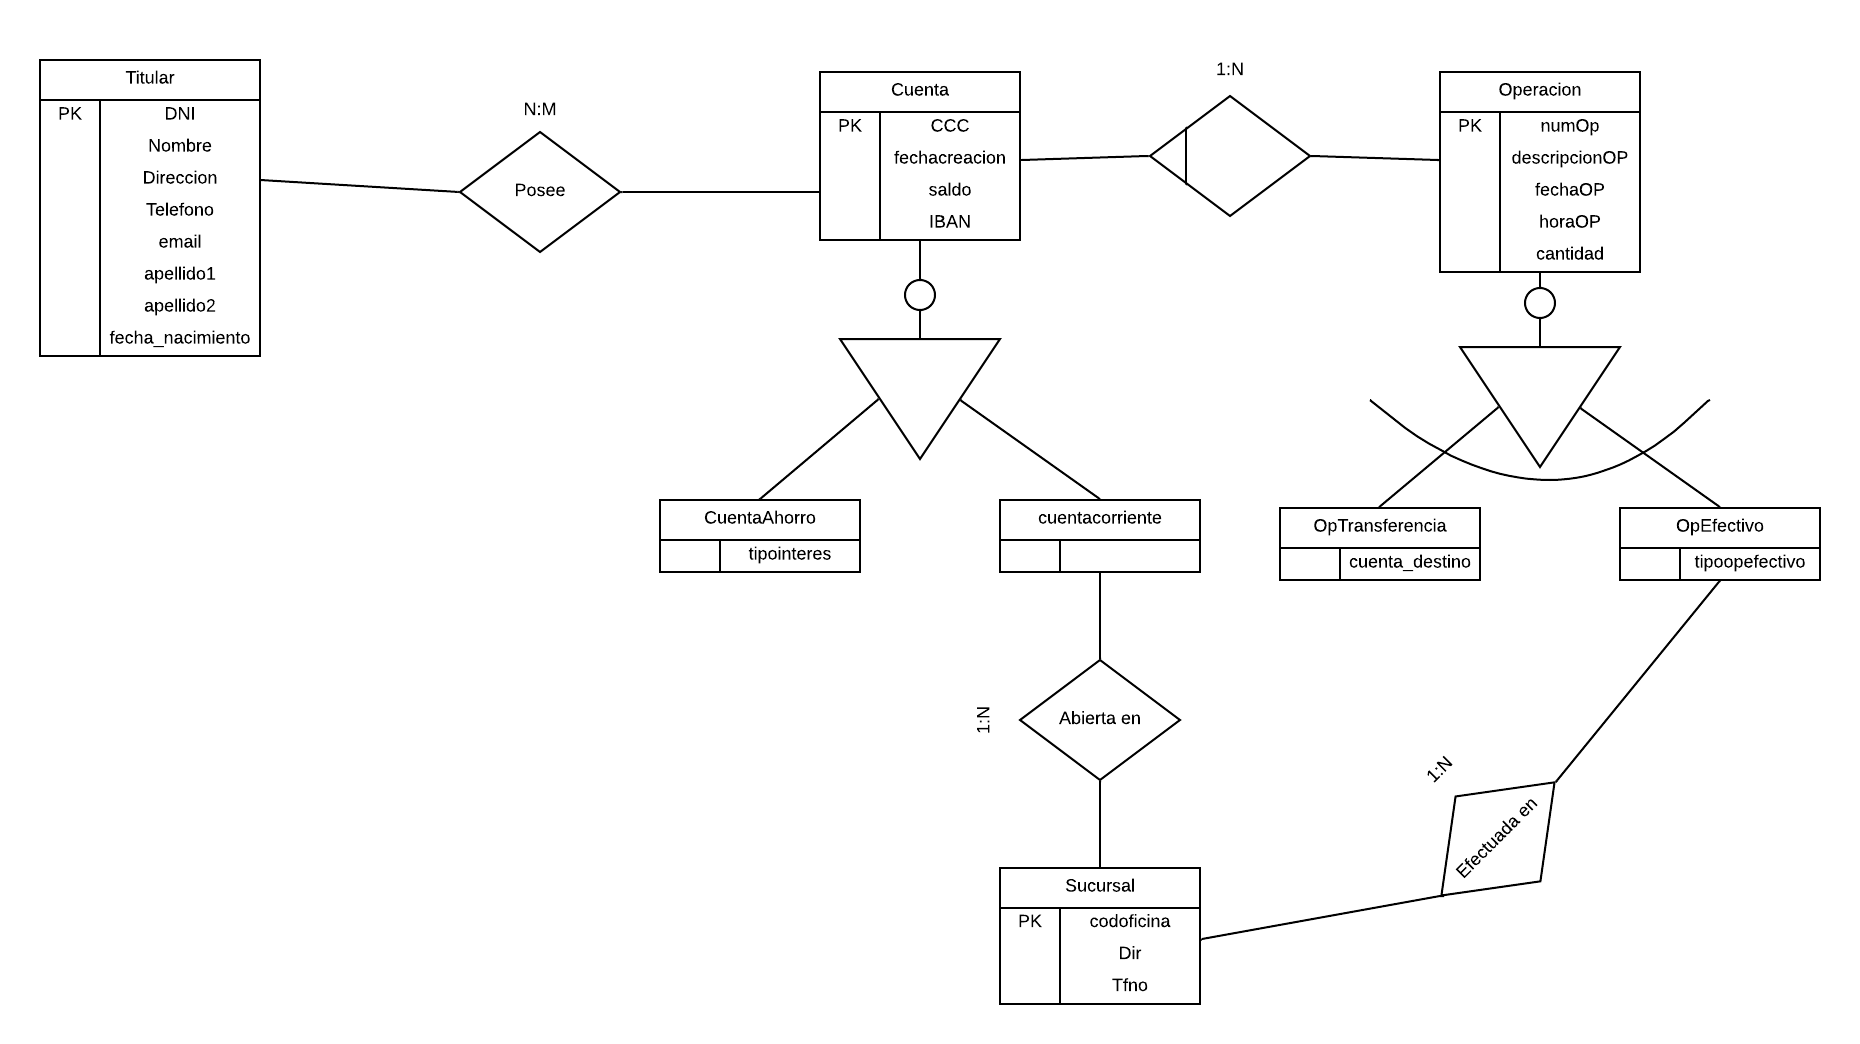
\includegraphics[scale=0.55]{images/DiagramaGLOBAL.png}
\label{fig:er_banquete}
\caption{Diagrama E/R de la base de datos de Banquete}
\end{figure}\\

La entidad \emph{Titular} es la que recogerá a todos los clientes de ambas bases, y contendrá toda su información, incluyendo la \textit{direccion}. Se ha optado por introducir este dato como un atributuo más de la tabla en lugar de crear una entidad con las direcciones. La dirección contendrá la calle, el piso, número y código postal. En el caso de \emph{Banquito} venía en un atributo, pero en el caso de \emph{Banquete}, se disponía en dos entidades, \textit{Dirección} y \textit{CodPostal}, esto se ha unificado en un atributo a través de la consulta ralizada a la hora de crear la vista con la siguientes sentencias:

\begin{lstlisting}
CREATE OR REPLACE VIEW titular_view AS
(
	-- BANQUITO
	-- Seleccionamos los atributos que queremos mostrar con sus respectivos
	-- nombres
	SELECT c.DNI as DNI, 
		c.nombre as NOMBRE,
		regexp_substr(c.apellido, '^[a-zA-Z]+\w|^[a-zA-Z]+$') APELLIDO1,
		regexp_substr(c.apellido, ' .*$') APELLIDO2,
		c.direccion as DIRECCION,
		TO_CHAR(c.telefono) as TELEFONO,
		c.email as EMAIL, 
		-- calculamos la edad ya que no disponemos de la fecha de 
		-- nacimiento, sino la edad en el momento de registro
		TO_DATE(sysdate-c.edad*365) as FECHA_NACIMIENTO
	FROM Cliente c
)
UNION
(
	-- BANQUETE
	-- Seleccionamos los atributos que queremos mostrar con sus respectivos
	-- nombres
	SELECT	t.DNI as DNI,
	t.nombre as NOMBRE, 
		t.apellido1 as APELLIDO1,
		t.apellido2 as APELLIDO2,
		d.calle || ', numero ' || d.numero || ', piso ' || d.piso 
			|| ', ' || d.ciudad || ', '
			|| (
				-- buscamos en codpostal el código correspondiente
				-- a la calle y ciudad que estamos mostrando
				SELECT distinct cp.codpostal 
				FROM codpostal@schema2bd2 cp 
				WHERE cp.calle = d.calle AND
					cp.ciudad = d.ciudad
			) 
			as DIRECCION,
		t.telefono as TELEFONO,
		-- no disponen de atributo email en banquete
		null as EMAIL,
		t.fecha_nacimiento as FECHA_NACIMIENTO
	FROM titular@schema2bd2 t 
		JOIN direccion@schema2bd2 d ON
			t.direccion = d.id_direccion
);
\end{lstlisting}
Para \emph{Banquito }simplemente se cogen los datos de la tabla \textit{Cliente} y se nombra las columnas siguiendo el esquema de \emph{Banquete}, de esta manera sus usuarios se sentirán mas cómdos. En cambio en la consulta a \emph{Banquete}, debemos realizar un \textit{join} con la tabla \textit{dirección} y  \textit{titular}, ya que el último contiene una clave ajena de dirección. Para obtener la dirección completa se concatenan los atributos de la tabla y para obtener el código posta, se hace a través de una consulta con la ciudad y la calle deseada.\\

La entidad \emph{Cuenta} contendrá tanto las cuenta corrientes como las cuentas de ahorro. Esta dispone de una relación \textit{posee} con titular con cardinalidad N:M, con esta relación vinculamos las cuenta con sus titulares. Para ello se realiza la siguiente vista:\\
\begin{lstlisting}
CREATE OR REPLACE VIEW Posee_view AS
    (
        SELECT p.DNI as TITULAR, to_char(p.Num_cuenta) AS CCC
        FROM Poseer p
    )
    UNION
    (
        select c1.titular, c1.CCC
        from cuenta@schema2bd2 c1
    );
\end{lstlisting}
Se realiza una unón con la tabla \textit{cuenta} de \emph{Banquete} y \textit{posee} de \textbf{Banquito}. \emph{Banquete} en su tabla \textit{cuenta } dispone de un atirbuto \textit{titular} que es el DNI del cliente al que pertenece esa cuenta (debido a la realación 1:N entre titular y cuenta). Para \emph{Banquito}  se ha tenido que obtener de la realación N:M posee que contine los DNIs asociados a sus cuentas.\\

\begin{lstlisting}
-- Cuenta (Padre)
CREATE OR REPLACE VIEW cuenta_view AS
    (
        SELECT TO_CHAR(c.Num_cuenta) AS CCC,
        c.Fecha_creacion as fechacreacion,
         c.saldo, 
         c.IBAN
        FROM Cuenta c
    )
    UNION
    (
        SELECT c1.CCC, 
        c1.fechacreacion, 
        c1.saldo, 
        (SELECT CONCAT(cod.codigo,cu.CCC) 
            from cuenta@schema2bd2 cu, codentidades@schema2bd2 cod
            where  cod.banco='Banquete' AND cu.CCC = c1.CCC) AS IBAN
        FROM cuenta@SCHEMA2BD2 c1
    );
\end{lstlisting}
Para crear la tabla de \textit{cuenta}, se hace una unión con cuenta de \emph{Banquito} y \emph{Banquete }, con la peculiaridad de que este último no contiene el IBAN y este se debe de obtener a través de una consulta a la tabla \textit{CodEntidades}.\\
Cuenta será la clase padre de una generalización total no exclusiva, sus hijos serán \textit{Cuenta Ahorro}, que dispondrá de una tributo \textit{tipo interés }que la diferencia de \textit{Cuenta Corriente}, además esta tiene una relaciuón 1:N con Sucursal, debido a que en ambos esquemas se encuentra de esta manera. Las vistas creadas son muy simples, basicamente se cogen los atributos y se renombran según el esquema de \emph{Banquete}.
\begin{lstlisting}
-- Cuenta Corriente
CREATE OR REPLACE VIEW cuenta_corriente_view AS
    (
        SELECT to_char(cc.ID_cuenta) AS CCC, cc.ID_sucursal AS SUCURSAL_CODOFICINA
        FROM Cuenta_Corriente cc
    )
    UNION
    (
        SELECT cc1.CCC, cc1.SUCURSAL_CODOFICINA
        FROM cuentacorriente@SCHEMA2BD2 cc1
    );

-- Cuenta_ahorrro
CREATE OR REPLACE VIEW cuenta_ahorro_view AS
    (
        SELECT to_char(cc.ID_cuenta) AS CCC, cc.Interes AS TipoInteres
        FROM Cuenta_ahorro cc
    )
    UNION
    (
        SELECT cc1.CCC, cc1.TIPOINTERES
        FROM cuentaahorro@SCHEMA2BD2 cc1
    );
\end{lstlisting}

La entidad \textit{Sucursal} es igual en ambos bancos, por lo que no exige gran dificultad realizar la unión. 
Además como se ha visto antes, hay una relación entre \textit{Cuenta Corriente} y \textit{Sucursal} de tipo 1:N, pero es cuenta corriente quien contiene la calve ajean de la sucursal en la que se abrió dicha cuenta.\\
Para la vista se realizan las siguientes sentencias SQL:
\begin{lstlisting}
CREATE OR REPLACE VIEW sucursal_view AS 
	(
		SELECT s.codigo AS codoficina, s.direccion AS dir, s.telefono AS tfno
		FROM Sucursal s
	)
	UNION
	(
		SELECT s1.codoficina, s1.dir, s1.tfno
		FROM sucursal@SCHEMA2BD2 s1
	);
\end{lstlisting}
La entidad \textit{Operación} (\textit{Transaccion} en \emph{Banquito}) es una entidad débil respecto a \textit{Cuenta} ya que depende de esta, en existencia y en identificación. Sin embargo, esto se soluciona con la relación entre Cuenta y Operación, de tipo 1:N, donde se propaga la clave de cuenta a Operación, eliminando de esta forma este problema. Cabe destacar que \textit{Operacion} es la entidad padre de una generalización total exclusiva, distinguiendo entre operaciones de trasnferencia y operaciones de efectivo. De esta manera se respeta el esquma de \emph{Banquete}. \\
En cuanto a \emph{Banquito}, en su diseño no se contempló la posibilidad de que una transferencia se realizase con una cuenta ajena que no estuviese registrada, por esta razón la tabla correspondiente a \textit{OpTrasnferencia} que es \textit{Transferencia} dispone de una relación 1:N con \textit{Cuenta} en el diseño de \emph{Banquito}. 
Para resolver la incosistencia del esquema de \emph{Banquete}, en el que una operación de efectivo contiene el código de la sucursal con un simple \textit{check} sin ser una referencia, se ha optado por una relación 1:N \textit{efectuado en } entre \textit{OpEfectivo} y \textit{Sucursal}, con esto se soluciona la incosistencia y se sigue el modelado.
Para obtener la vista se realiza la siguiente consulta:

\begin{lstlisting}
CREATE OR REPLACE VIEW operacion_view AS
(
	SELECT *
	FROM (
		SELECT t1.num_transaccion AS numop, t1.descripcion AS descripcionop, 
		t1.fecha AS fechaop, TO_CHAR(t1.fecha, 'HH24:MI') AS horaop, 
		t1.importe AS cantidadop, TO_CHAR(t1.NUM_CUENTA_REALIZANTE) AS ccc
		FROM TRANSACCION t1
	)
	UNION
	(
		SELECT op.num_transaccion AS numop, op.descripcion AS descripcionop,
		 op.fecha AS fechaop, TO_CHAR(op.fecha, 'HH24:MI') AS horaop,
		  op.importe AS CANTIDADOP, TO_CHAR(op.NUM_CUENTA_REALIZANTE) AS ccc
		FROM operacion op
	)
)
UNION
(
	SELECT o.numop, o.descripcionop, o.fechaop, o.horaop, o.cantidadop, o.ccc
	FROM operacion@SCHEMA2BD2 o
);
\end{lstlisting}
Respetando el esquema de \emph{Banquete}, realizamos una unión con \textit{Transacción} y \textit{Operación} en \emph{Banquito}, 
\begin{huge} pendiente \end{huge}\\
Para \textit{OpTransferencia}, se realiza una unión, con la tabla \textit{Transaccion} de \emph{Banquito} y con un \textit{join} entre \textit{Operacion} y \textit{OpTransferencia}  en el esquema de \emph{Banquete} cogiendo únicamente aquellas operaciones que pertenecen a una transferencia.

\begin{lstlisting}
CREATE VIEW optransferencia_view AS
(
	SELECT t1.num_transaccion AS numop, t1.descripcion AS descripcionop, 
			t1.fecha AS fechaop, 
			TO_CHAR(t1.fecha, 'HH24:MI') AS horaop, 
			t1.importe AS cantidadop, 
			TO_CHAR(t1.NUM_CUENTA_REALIZANTE) AS ccc,
			TO_CHAR(t1.NUM_CUENTA_BENEFICIARIO) AS cuentadestino
	FROM TRANSACCION t1
)
UNION
(
	SELECT o.numop, o.descripcionop, o.fechaop, o.horaop, o.cantidadop, 
	o.ccc, ot.cuentadestino
	FROM operacion@SCHEMA2BD2 o JOIN optransferencia@SCHEMA2BD2 ot 
		ON o.numop = ot.numop AND o.ccc = ot.ccc
);
\end{lstlisting}
Para \textit{OpEfectivo} ocurre lo mismo que con la anterior tabla, la consulta es igual, simplemente se cambia la tabla de \textit{Transaccion } por \textit{Operación} en \emph{Banquito}, y en \emph{Banquete} la tabla de \textit{OpTransferencia } por \textit{OpEfectivo}.
\begin{lstlisting}
CREATE VIEW opefectivo_view AS
	(
		SELECT t1.num_transaccion AS numop, t1.descripcion AS descripcionop, 
				t1.fecha AS fechaop, 
				TO_CHAR(t1.fecha, 'HH24:MI') AS horaop, 
				t1.importe AS cantidadop, 
				TO_CHAR(t1.NUM_CUENTA_REALIZANTE) AS ccc,
				t1.tipo AS tipoopefectivo,
				t1.codigo AS sucursal_codoficina
		FROM OPERACION t1
	)
	UNION
	(
		SELECT o.numop, o.descripcionop, o.fechaop, o.horaop, o.cantidadop,
			 o.ccc, oe.tipoopefectivo, oe.sucursal_codoficina
		FROM operacion@SCHEMA2BD2 o 
			JOIN opefectivo@SCHEMA2BD2 oe 
				ON o.numop = oe.numop AND o.ccc = oe.ccc
	);
\end{lstlisting}
\section{Parte 2 - Enunciado de un problema de diseño de bases de datos}

Se desea diseñar una base de datos para gestionar la información inherente a un hospital. En el hospital trabajan médicos y enfermeros. Los médicos tienen asignados una serie de pacientes. Los enfermeros tienen asignada una planta.\\
%Los pacientes ingresan en el hospital a partir del servicio de urgencias, y tras examinarles se les asigna a una planta.\\
La información sobre los trabajadores del hospital deberá contener información sobre su DNI, nombre, apellidos, fecha de nacimiento, dirección, teléfono de contacto. Los médicos deberán almacenar su especialidad y su número de colegiado. Los enfermeros almacenarán el servicio al que están asignados (planta, hematología, diálisis...).\\
Nuestro hospital está dividido en plantas, cada planta alberga pacientes ingresados y almacena la información relativa al uso destinado para esa planta.\\
Los pacientes almacenan su DNI, nombre, apellidos, fecha de nacimiento, dirección y teléfono. Disponemos de un historial clínico que almacena la información sobre los diagnósticos realizados a los pacientes.

\textbf{Poner aqui ese enunciado que hemos redactado}

\section{Parte 2- Esquema conceptual para el problema enunciado}

Para la realización del esquema conceptual de este problema, y pensando en su futura tarea de integración, se han realizado dos esquemas conceptuales con una semántica similar para el problema descrito anteriormente. Se ha tomado esta decisión para dificultar la tarea de integración entre las dos bases de datos.\\

El primer diagrama (Figura \ref{fig:er_parte2_1}) refleja el problema enunciado anteriormente. En el mismo podemos observar que debido a que los médicos, enfermeros y pacientes comparten ciertos atributos (\emph{DNI}, Nombre, apellidos, dirección, teléfono...) se ha llegado a la conclusión de que debía existir una entidad común, \emph{Personal}..\\
Dirección se ha representado como una entidad debido a que como clave primaria son un conjunto de atributos (Calle, bloque, número de piso y código postal).\\
La entidad diagnóstico es débil respecto a \emph{Paciente} debido a que depende en identificación y existencia de ella.\\
Para representar los \emph{Paciente} que han sido ingresados en cada una de las \emph{Plantas} se ha diseñado la relación \emph{N:M} \emph{Ingresos}, la cual posee un atributo Fecha, que representa el momento en el que el paciente fue ingresado en dicha planta.\\
Dado que los médicos tienen varios pacientes, y un paciente puede tener varios médicos, se ha diseñado una relación \emph{M:N} entre \emph{Médicos} y \emph{Pacientes}.\\

El segundo diagrama (Figura \ref{fig:er_parte2_2}) refleja el problema enunciado anteriormente. En el mismo podemos observar que debido a que los médicos y enfermeros comparten ciertos atributos (\emph{DNI}, Nombre, apellidos, dirección, teléfono...) se ha llegado a la conclusión de que debía existir una entidad común, \emph{Personal}.\\
Por otra parte, los diagnósticos realizados por los pacientes forman su historia clínica. La entidad \emph{Diagnóstico} es una entidad débil ya que depende en identificación y en existencia de \emph{Paciente}.\\
Los pacientes ingresan en plantas, por lo tanto, se ha diseñado una entidad \emph{Ingreso} que refleja el ingreso de un paciente determinado en una planta determinada. Esta entidad es débil ya que un paciente puede encontrarse con varios ingresos a lo largo de su vida. Por lo tanto, un ingreso depende de la planta, el paciente y, las fechas de ingreso y de alta.\\
Dado que los médicos tienen varios pacientes, y un paciente puede tener varios médicos, se ha diseñado una relación \emph{M:N} entre \emph{Médicos} y \emph{Pacientes}.

\textbf{Poner aquí los dos esquemas ER y explicar que se ha tomado esta decisión para dificultar la integración.}

\section{Parte 2 - Esquema lógico 1 para el problema enunciado}

En la traducción del esquema conceptual al esquema lógico del primer modelo se han traducido la generalización entre personal, médicos, enfermeros y pacientes con una generalización en la que toda la información es almacenada en las tablas \emph{hijas} (Médico, Enfermero y Paciente), sin crear una tabla \emph{Personal}.\\
Para la traducción de la entidad dirección, debido a que al tener una relación 1:N con \emph{Personal} debe almacenarse su clave primaria ( la cual es un conjunto de atributos), se ha decidido crear una clave subrogada como identificador primario de la tabla \emph{Dirección}.\\
Para modelar el histórico de diagnósticos sobre un paciente se ha creado una tabla \emph{Diagnóstico} con una restricción de clave ajena hacia la tabla \emph{Pacientes}, por lo tanto se ha modelado la entidad débil.\\
Las relaciones N:M (entre médicos y pacientes, enfermeros y plantas y pacientes y plantas) se han traducido como nuevas tablas con restricciones de clave ajena entre las entidades relacionadas y los atributos de de la relación como atributos de las tablas.

\section{Parte 2 - Esquema lógico 2 para el problema enunciado}

En la traducción del esquema conceptual al esquema lógico del segundo modelo se han traducido la generalización entre personal, médicos y enfermeros con una generalización mixta, es decir, existirá una tabla \emph{Personal}, que almacenará los campos comunes a las tablas derivadas, y también existirán tablas para las derivadas, de tal forma que almacenarán sus campos propios.\\
Para modelar el histórico de diagnósticos sobre un paciente se ha creado una tabla \emph{Diagnóstico} con una restricción de clave ajena hacia la tabla \emph{Pacientes}, por lo tanto se ha modelado la entidad débil.\\
La tabla \emph{Ingreso} posee dos claves ajenas, una apuntando a una \emph{Planta} y otra a \emph{Paciente}, haciendo que los ingresos estén relacionados con las plantas y los pacientes,. Por lo tanto, un paciente distinto puede tener varios ingresos varias veces en una misma o distintinta planta a lo largo del tiempo en fechas distintas.\\
Para relacionar los médicos con los pacientes a los que tienen asignados, se ha traducido la relación \emph{M:N} en una nueva tabla \emph{Atendidos}, que almacenan las claves primarias de \emph{Médicos} y \emph{Pacientes}. Lo mismo ocurre entre \emph{Enfermeros} y \emph{Plantas}, se ha creado la tabla \emph{Asignados} que almacena las claves primarias de enfermeros y plantas.\\


\textbf{Haría falta meter los códigos en un anexo aunque sea?}
\textbf{Pues explicar las decisiones de diseño de este (PEDRO Y HAYK).}

\section{Parte 2 - Esquema global y su implementación en PostgreSQL}

Tras la traducción del esquema conceptual a los esquemas lógicos llega el turno de realizar la integración de ambos modelos lógicos en un solo esquema global que recoja las características de ambos esquemas lógicos.\\
Para ello, se ha compuesto el esquema global (Figura \ref{fig:er_parte2_global}). En este diagrama podemos observar que se encuentran características de ambos esquemas conceptuales. \\
De cara a la implementación de este esquema utilizando \emph{PostgreSQL} se han utilizado vistas con manteniendo los nombres de las entidades mostrados en el esquema global. Ya que las generalizaciones se habían planteado de una forma distinta sobre las traducciones de los esquemas lógicos, se han realizado vistas que permitan seguir obteniendo toda la información que se podía consultar utilizando el \emph{Esquema lógico 1}. Por lo tanto, consultando la vista \emph{Personalview} obtendremos todos los datos comunes a las entidades que se derivan de la misma, tal y como se plantea en el \emph{Esquema lógico 2}. Para cada entidad derivada se han diseñado vistas para acceder a sus tuplas insertadas. En el caso de estas vistas, se mantiene el un conjunto de valores similar al utilizado por el esquema lógico 1.\\
Una diferencia de integración entre ambos esquemas ha sido la dirección. Esta entidad no aparece en el esquema lógico 2, y por lo tanto para facilitar su integración se ha eliminado como una entidad y se ha añadido como un atributo más a la entidad \emph{Personal}. Algo similar ocurre con \emph{Apellido1} y \emph{Apellido2}, dos atributos que se encuentran presentes en el esquema lógico 2 pero que se encuentran unificados en el esquema lógico 1. En este caso se ha tomado la decisión de unificarlos bajo una columna en la vista (\emph{Apellidos}).\\
En el caso de la entidad \emph{Ingreso} existente en el esquema lógico 2, se ha tomado la decisión de mantenerla ya que existe una relación en el esquema lógico 1 que mantiene la misma semántica, aunque no cuenta con todos los atributos necesarios (fecha de alta), en ese caso se asignará el valor \emph{NULL} para aquellos atributos con los que no se cuente información.\\

En el apartado técnico, se ha utilizado la herramienta \emph{dblink\footnote{\url{https://www.postgresql.org/docs/10/contrib-dblink-function.html}}} de \emph{PostgreSQL} para realizar la conexión a la base de datos remota. Se realizará la integración suponiendo que la base de datos local es la correspondiente implementación del \emph{Esquema lógico 1}. Para mantener la implementación del \emph{Esquema lógico 2} se ha utilizado el servicio \emph{ElephantSQL\footnote{\url{https://www.elephantsql.com/}}} para obtener una instancia de \emph{PostgreSQL} en la nube.\\
Para realizar la conexión con la base de datos remota se ha ejecutado la siguiente consulta, la cual guarda los datos de la conexión bajo el alias ``remota''.

\begin{lstlisting}
select * from dblink_connect('remota',
 'host=kandula.db.elephantsql.com  dbname=** user=** password=**');
\end{lstlisting}

Tras ejecutar esta sentencia, se habra realizado la conexión con la base de datos ubicada en \emph{kandula.db.elephant.sql}.\\
Para ejecutar una consulta sobre \emph{dblink} podemos utilizar una forma similar a la siguiente:

\begin{lstlisting}
select DNI, Nombre, Apellido1 || ', ' || Apellido2 as "Apellidos",
 Telefono, Direccion, Especialidad, Num_Colegiado as "NumColegiado"
from dblink('remota', 
'select pe."DNI", pe."Nombre", pe."Apellido1", pe."Apellido2",' || 
' pe."Telefono", pe."Direccion",' || 
' m."Especialidad", m."Num_Colegiado"' ||
' from "Personal" pe join "Medicos" m on pe."DNI"=m."DNI"') 
 as (DNI varchar, Nombre varchar, Apellido1 varchar,
  Apellido2 varchar, Telefono varchar,
  Direccion varchar, Especialidad varchar, Num_Colegiado varchar);
\end{lstlisting}

Con esta consulta, obtendremos toda la información de los médicos, junto con sus datos de personal de la base de datos de la base de datos remota.\\
Se puede observar que es necesario establecer de manualmente los campos de la consulta tras la cláusula \emph{as}. Con esto se puede realizar conversiones de tipos de forma implícita, ya que si no habría que realizarlas en la primera parte de la consulta utilizando los casts\footnote{\url{https://www.postgresqltutorial.com/postgresql-cast/}} explícitos de \emph{PostgreSQL}.\\

Tras realizar la conexión con la base de datos remota y aprender a realizar consultas se va a proceder a integrar los esquemas. Para ello se van a utilizar vistas. El nombre de las vistas será igual al de las entidades de la Figura \ref{fig:er_parte2_global}.\\
La creación de las será similar al expuesto para el caso de \emph{Oracle}.
Por lo tanto, se procede a la creación de las mismas.

\begin{lstlisting}
create or replace view Personal_view as 
    (
        select p."DNI", 
         p."Nombre", 
         p."Apellidos", 
         p."NumContacto" as "Telefono", 
         d."Calle" || ',' || 
         d."NumBloque" || ', ' || 
         d."NumPiso" || ', ' || 
         d."CodPostal" as "Dirección"
        from "Medico" p join "Direccion" d on p."ID" = d."ID"
    )
    union
    (
        select p."DNI", 
         p."Nombre", 
         p."Apellidos", 
         p."NumContacto" as "Telefono", 
         d."Calle" || 
         ', ' || d."NumBloque" || 
         ', ' || d."NumPiso" || 
         ', ' || d."CodPostal" as "Dirección"
        from "Enfermero" p join "Direccion" d on p."ID" = d."ID"
    )
    union
    (
        select p."DNI",
         p."Nombre",
         p."Apellidos",
         p."NumContacto" as "Telefono",
         d."Calle" || ', ' ||
         d."NumBloque" ||
         ', ' || d."NumPiso" ||
         ', ' || d."CodPostal" as "Dirección"
        from "Paciente" p join "Direccion" d on p."ID" = d."ID"
    )
    union
    (
        select DNI, Nombre, Apellido1 || 
         ', ' || Apellido2 as "Apellidos", 
         Telefono, Direccion
		from dblink('remota',
		 'select "DNI", "Nombre", "Apellido1", "Apellido2",' ||
		  ' "Telefono", "Direccion" from "Personal"') 
		  as (DNI varchar, Nombre varchar, Apellido1 varchar, 
		  Apellido2 varchar, Telefono varchar, Direccion varchar)
    )
    union
    (
        select DNI, Nombre, Apellido1 || 
        ', ' || Apellido2 as "Apellidos", 
        Telefono, Direccion
		from dblink('remota', 
		 'select "DNI", "Nombre", "Apellido1", "Apellido2", ' || 
		  '"Telefono", "Direccion" from "Pacientes"') 
		  as (DNI varchar, Nombre varchar, Apellido1 varchar,
		  Apellido2 varchar, Telefono varchar, Direccion varchar)
    );
\end{lstlisting}


Con esta vista obtenemos al personal, de la misma forma que se obtendrían con el esquema lógico 2, pero añadiendo a los pacientes, cosa que venía incluida en el esquema lógico 1.\\
No obstante, podemos obtener las entidades derivadas de personal con el formato especificado en el esquema lógico 1 utilizando la siguiente vista (en el caso de médicos):


\begin{lstlisting}
create or replace view Medico_view as
    (
        select p."DNI", p."Nombre", p."Apellidos",
         p."NumContacto" as "Telefono",
          d."Calle" || ', ' || d."NumBloque" ||
          ', ' || d."NumPiso" || ', ' ||
          d."CodPostal" as "Dirección",
          p."Especialidad", p."NumColegiado"
        from "Medico" p join "Direccion" d on p."ID" = d."ID"
    )
    union
    (
        select DNI,
         Nombre, Apellido1 || ', ' || Apellido2 as "Apellidos",
         Telefono, Direccion,
         Especialidad,
         Num_Colegiado as "NumColegiado"
		from dblink('remota', 'select pe."DNI", pe."Nombre",' ||
		 ' pe."Apellido1", pe."Apellido2", pe."Telefono", ' ||
		 'pe."Direccion", m."Especialidad", m."Num_Colegiado" ' ||
		 'from "Personal" pe join "Medicos" m on pe."DNI"=m."DNI"') 
		 as (DNI varchar, Nombre varchar, Apellido1 varchar,
		  Apellido2 varchar, Telefono varchar, Direccion varchar,
		  Especialidad varchar, Num_Colegiado varchar)
    );
\end{lstlisting}


Para obtener los resultados sobre las entidades \emph{Enfermeros} y \emph{Pacientes} se pueden utilizar las vistas: \emph{Enfermeroview} y \emph{Pacienteview}, respectivamente.\\
Para el acceso a los datos de la entidad \emph{Ingreso} podemos utilizar \emph{Ingresosview}, definida de la siguiente forma.\\

\begin{lstlisting}
create or replace view Ingresos_view as
    (
        select "NumPlanta", "DNI", "Fecha" as "Fecha_Ingreso", 
         NULL as "Fecha_Alta"
        from "Ingresos"
    )
    union
    (
        select NumPlanta, DNI, Fecha_Ingreso, Fecha_Alta
        from dblink('remota', 
         'select "DNI", "Num_Planta", "Fecha_Ingreso", ' || 
          '"Fecha_Alta" from "Ingresos"') 
          as (DNI varchar, NumPlanta int, Fecha_Ingreso date,
           Fecha_Alta date)
    );
\end{lstlisting}

En esta vista se puede observar como el esquema lógico 1 no contaba con una fecha de alta el la relación \emph{Ingresos}, y por lo tanto ha tenido que ser sustituida por el valor \emph{NULL}.\\

\textbf{{\LARGE ¿QUERÉIS QUE SIGA EXPLICANDO EL RESTO DE VISTAS O CON ESTO ES SUFICIENTE?}}

\textbf{Puse aquí tenemos la incertidumbre de si querrán que sean vistas o una base de datos completa, pero de todas formas habrá que explicar las decisiones de diseño.}

\section{Actualizaciones de datos sobre el esquema global}
El esquema global es una representación que unifica los esquemas lógicos de dos o más bases de datos. Se utiliza cuando las bases de datos en cuestión tienen cierta relación e interesa obtener información de ambas mediante un solo acceso, en vez de acceder por separado a las mismas. Con esta representación global se intenta ajustar las distintas entidades, relaciones y atributos de las bases participantes para que el esquema global sea lo más parecido posible a las mismas. 
En nuestro caso, tanto para el apartado de \textit{Oracle} como el de \textit{PostgreSQL}, las bases de datos que componen los respectivos esquemas globales son lógicamente diferentes entre sí. Es por ello que toda la información se almacena en cada una de ellas por separado y para representar el esquema global se crean vistas que recogen la información de las mismas y la  muestran de una forma unificada. De esta manera, si se quisiera modificar información en el esquema global, podría dar problemas dado que, por un lado, como se ha mencionado anteriormente toda información se guarda en las bases componentes y por ello si se modifica la información de las vistas, el cambio no perdura en el tiempo. Por otro lado, si en lugar de utilizar vistas, se utilizaran tablas o vistas materializadas, de forma que se garantizara la persistencia de los cambios en el esquema global, cualquier modificación en el mismo debe transmitirse a la base correspondiente, es decir, se deberían programar \textit{Triggers} para garantizar la consistencia. Además de ser un trabajo complicado, las diferencias en la representación lógica de las bases implicaría, en algunos casos, una transofrmación de la información añadida/modificada. Por ejemplo, en el esquema global de \textit{Banquete} y \textit{Banquito} se representa la "Dirección" como una sola cadena. Si se añade un cliente relacionado con la base \textit{Banquete}, a la hora de actualizar la información en esta base, se observa que "Dirección" se representa en una tabla "Direccon" con distintos atributos, es decir, posee una representación lógica diferente. Para introducirlo en la base, se debería procesar la información y separar la cadena proveniente del esquema global en los distintos atributos de la tabla correspondiente de \textit{Banquete}, lo que sería un proceso ocioso y podría producir errores de inserción. 
En conclusión, tanto si el equema global se representa por medio de vistas o no, es recomendable utilizar el mismo únicamente para realizar consultas y realizar la inserción o modificación de datos en las bases componentes por separado 
\textbf{Viabilidad? Pues depende de dónde quieras guardarlo. Pero esto habrá que hablar.}\\
\\
\newpage


\section{Apéndice 1: Figuras}

\begin{landscape}
\begin{figure}
\centering
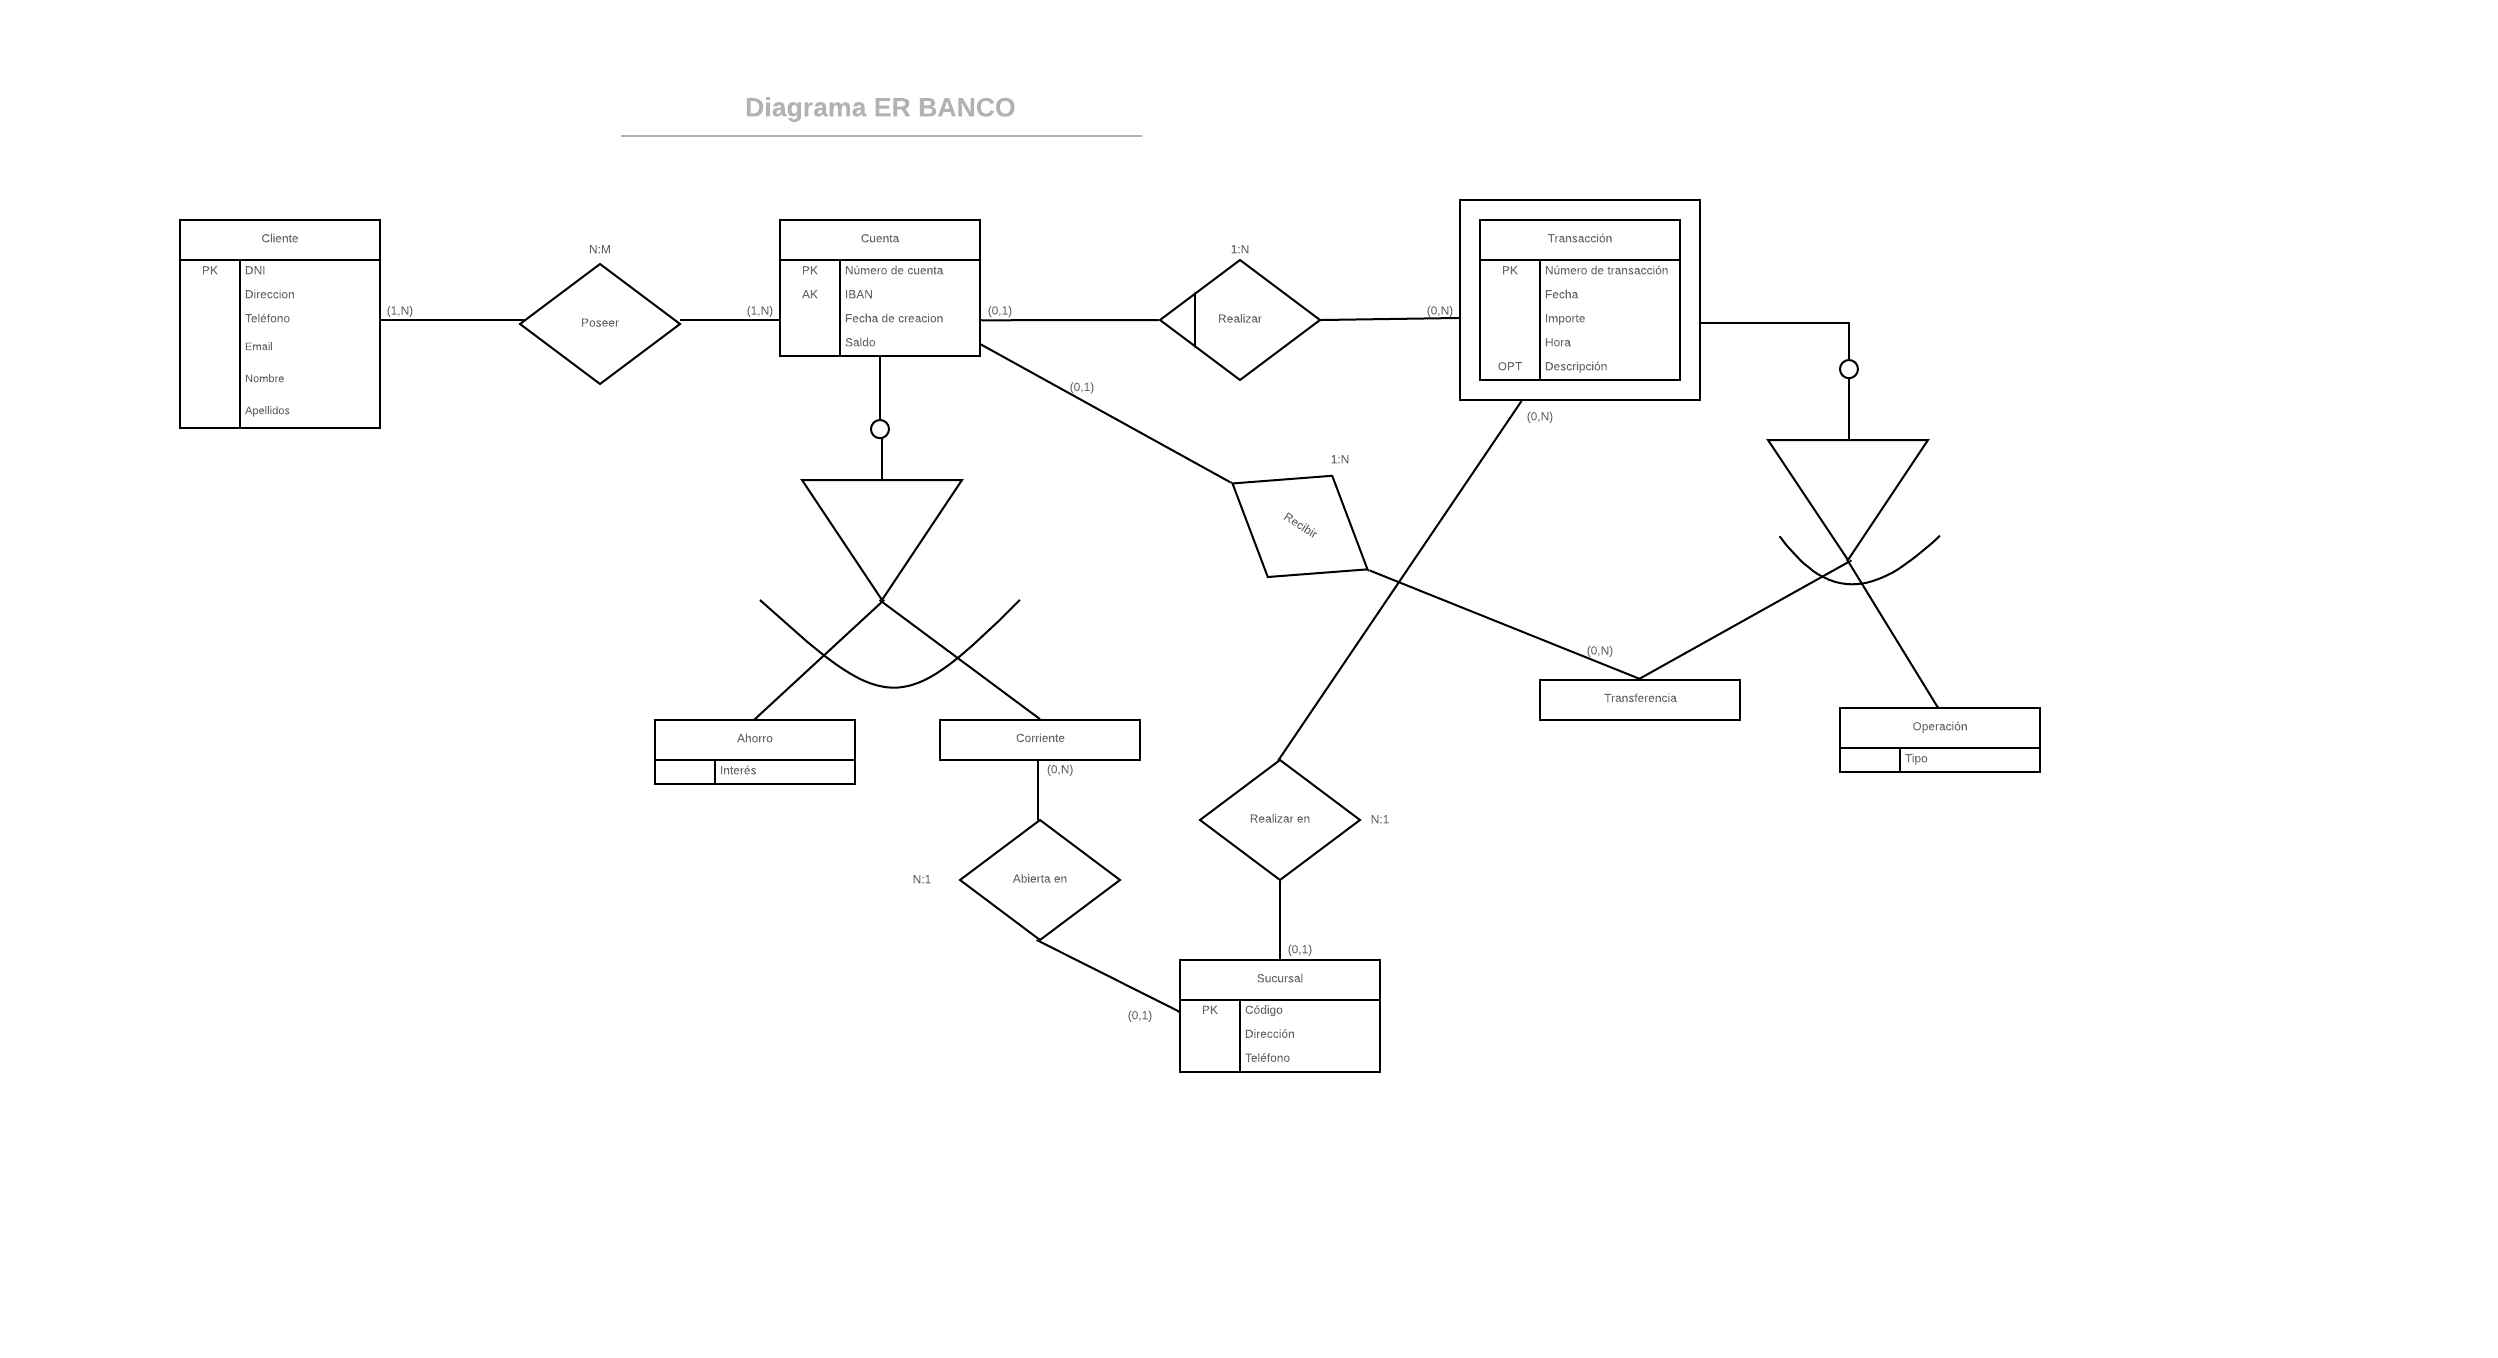
\includegraphics[scale=0.75]{images/er_practica1.png}
\caption{Esquema ER de la base de datos diseñada en la práctica 1}
\label{fig:er1}
\end{figure}
\end{landscape}




\newpage
\begin{landscape}
\begin{figure}
\centering
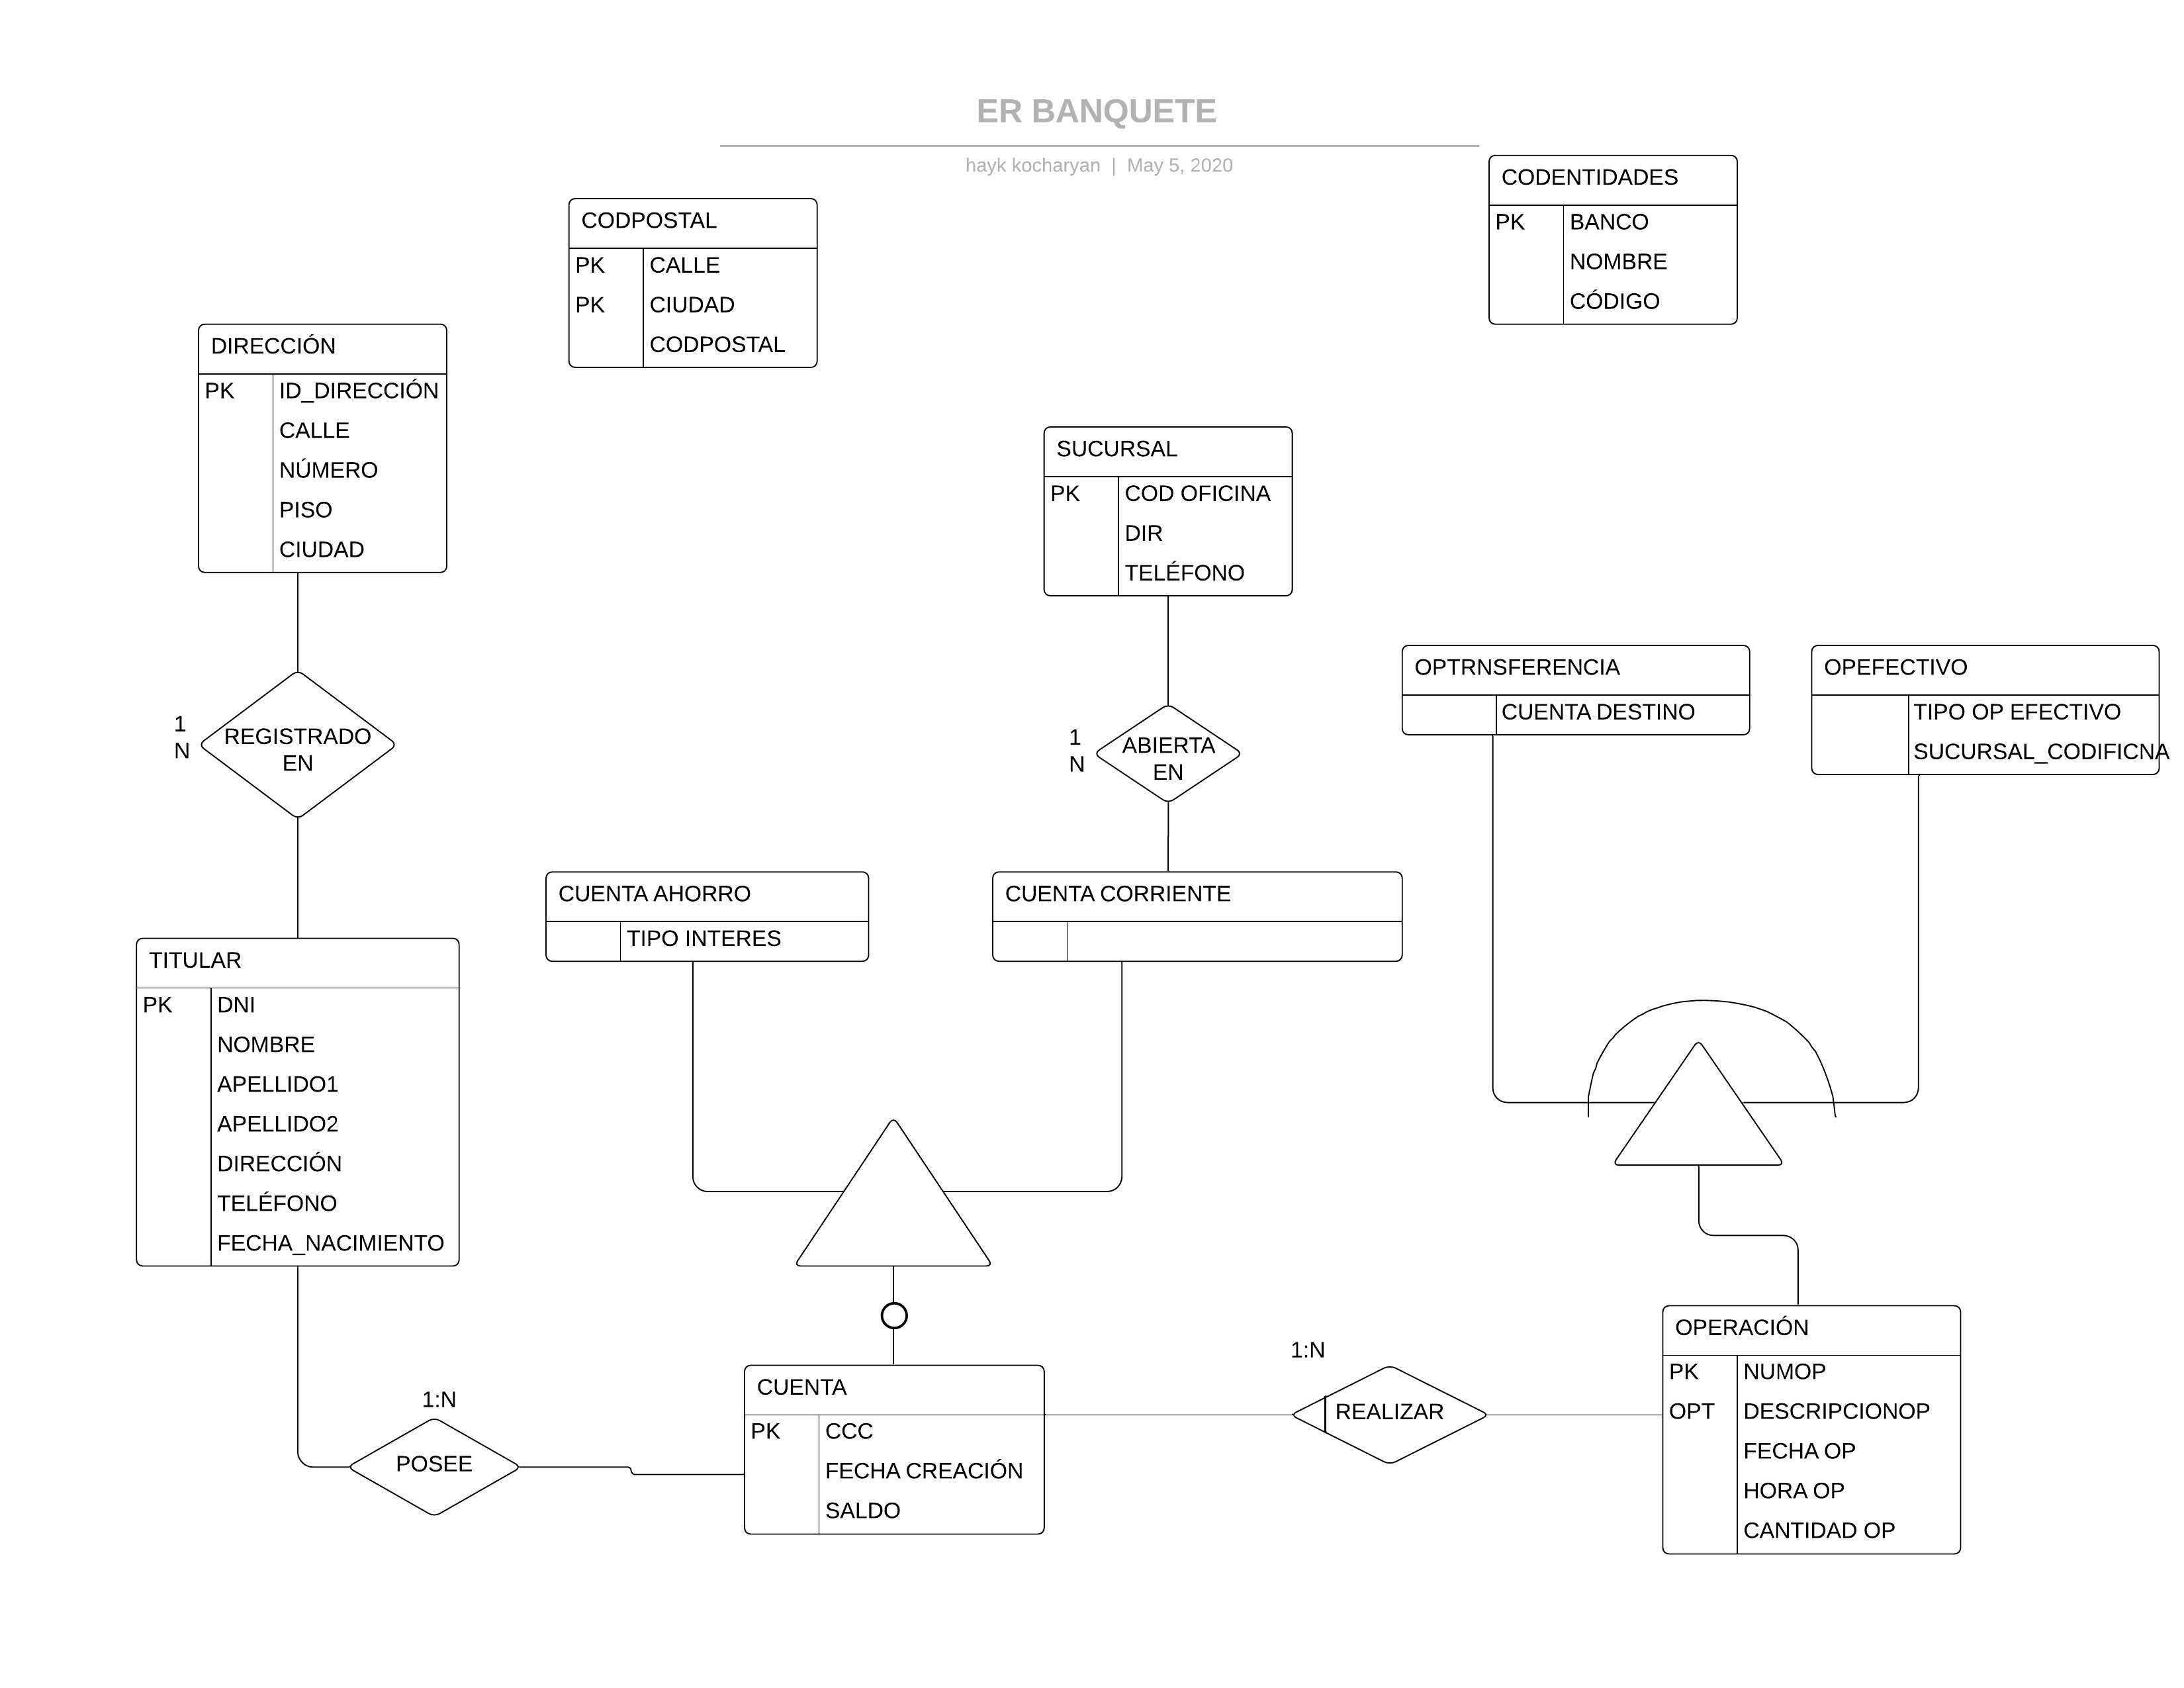
\includegraphics[scale=0.75]{images/ER_BANQUETE.jpeg}
\caption{Diagrama E/R de la base de datos de Banquete}
\label{fig:er_banquete}
\end{figure}
\end{landscape}
\pagebreak



%% DIAGRAMAS PARTE 2

\begin{landscape}
\begin{figure}
\centering
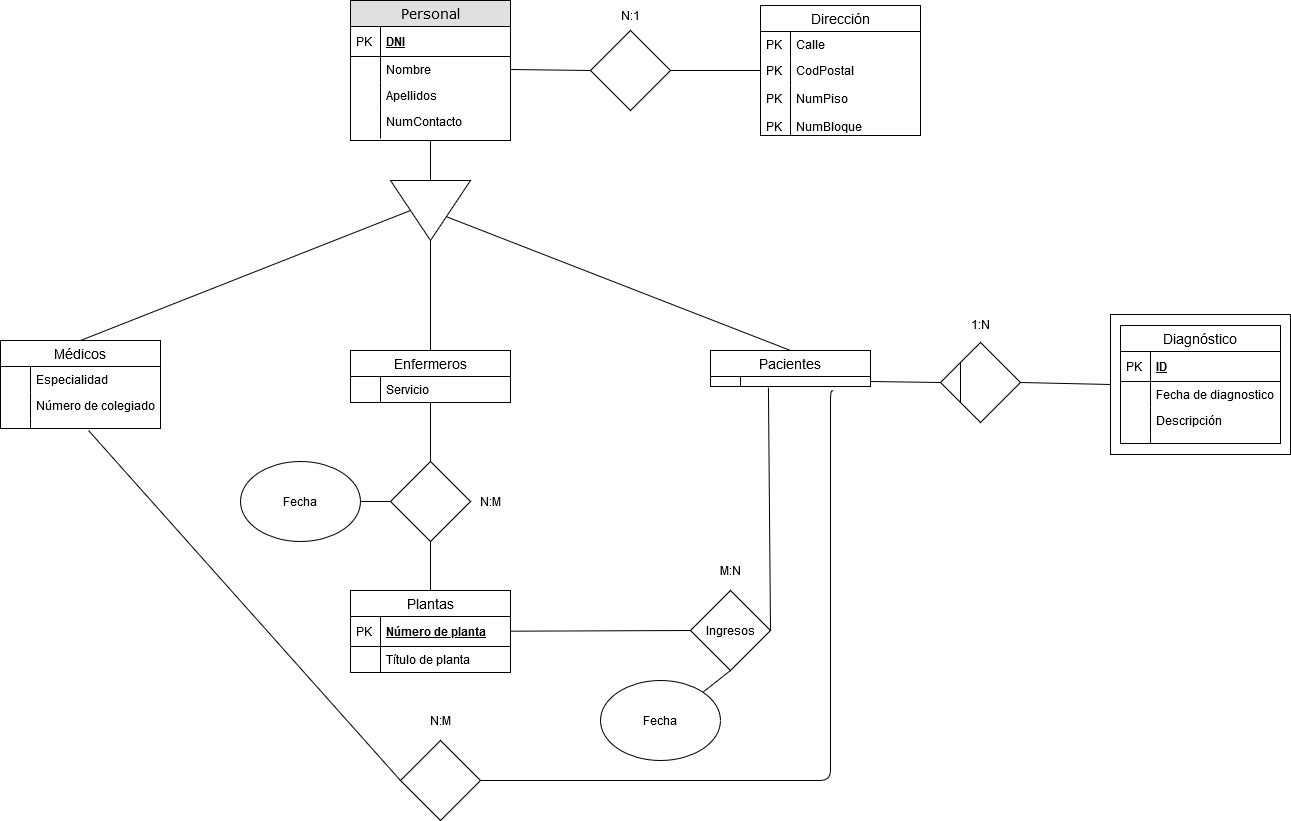
\includegraphics[scale=0.5]{images/er_parte2_1.jpg}
\caption{Diagrama ER de la primera solución sobre el problema descrito en la parte 2}
\label{fig:er_parte2_1}
\end{figure}
\end{landscape}

\begin{figure}
\centering
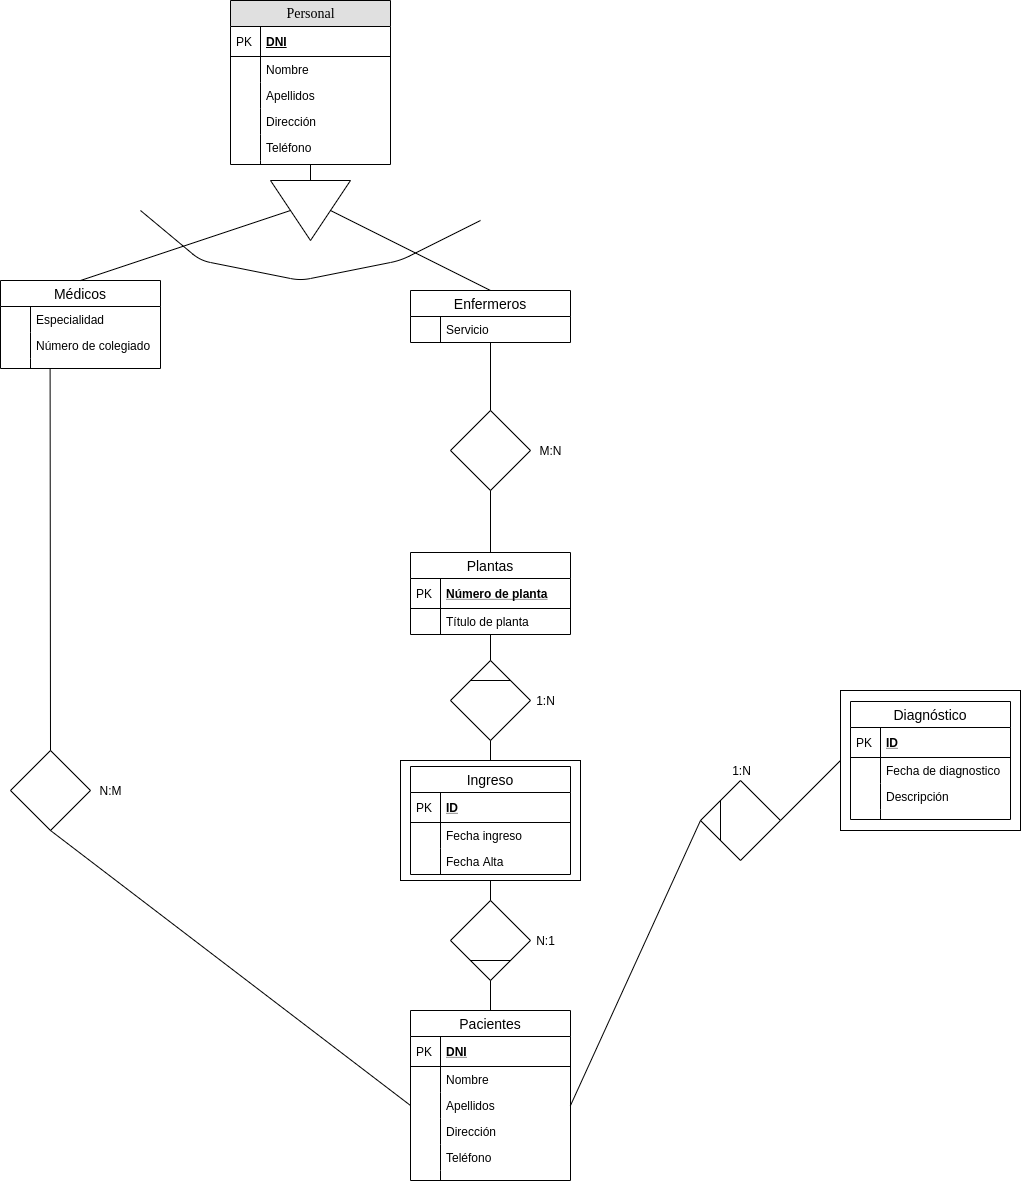
\includegraphics[scale=0.5]{images/er_parte2_2.png}
\caption{Diagrama ER de la segunda solución sobre el problema descrito en la parte 2}
\label{fig:er_parte2_2}
\end{figure}

\begin{landscape}
\begin{figure}
\centering
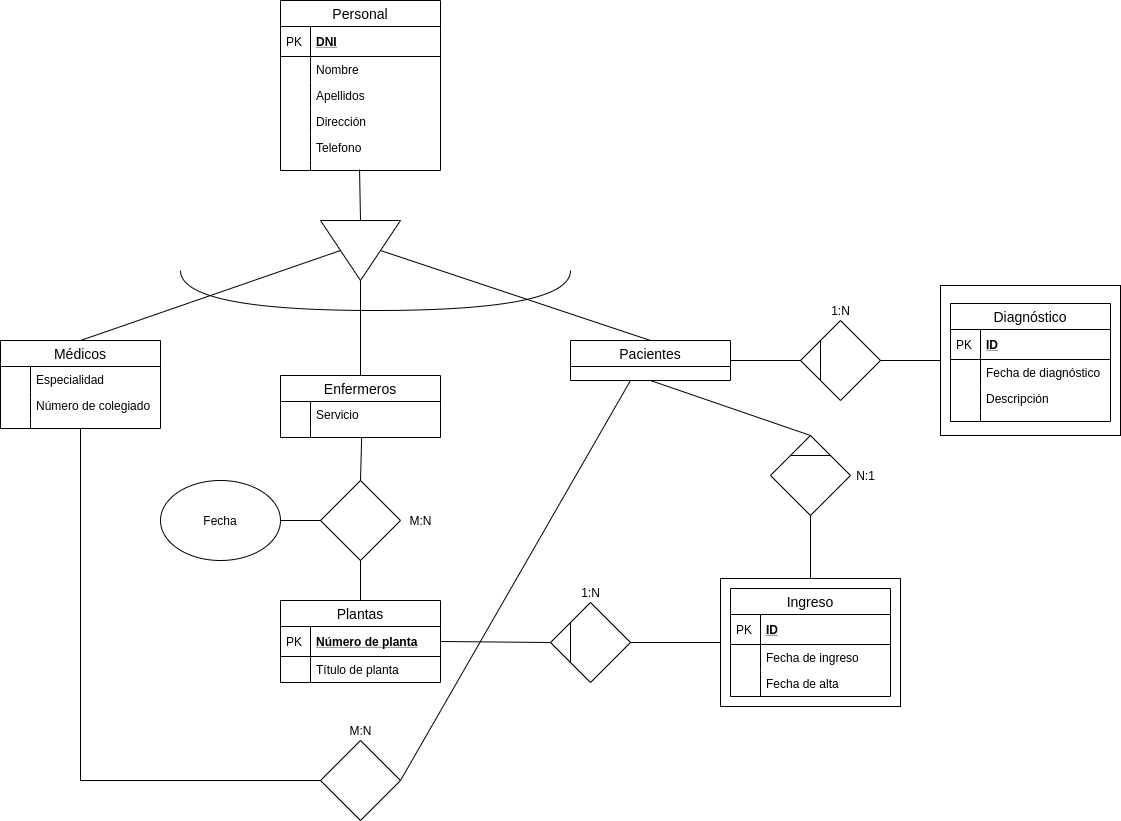
\includegraphics[scale=0.45]{images/global_parte2_practica3.png}
\caption{Diagrama ER global sobre la parte 2}
\label{fig:er_parte2_global}
\end{figure}
\end{landscape}


\end{document}
